The \textit{RDR\_nkz (Atlantic Conditions)} dataset was created by selecting parts of \textit{RDR\_nkz} dataset which have the 4 essential features in the range of what is present in the \textit{Atlantic} dataset.

First, for each feature, the \textit{Atlantic} distribution was checked to see in which value range the models were trained on. Then, the \textit{RDR\_nkz} plot was inspected, to determine candidate sections where the values were in the training range. Later, the sections where the candidates intersect for all features were chosen, and then concatenated to produce the \textit{RDR\_nkz (Atlantic Conditions)} dataset.

\clearpage
\subsubsection{True Wind Speed (TWS)}
The whole range of \textit{RDR\_nkz} is covered in the training set.

\begin{figure}[h]
\centering
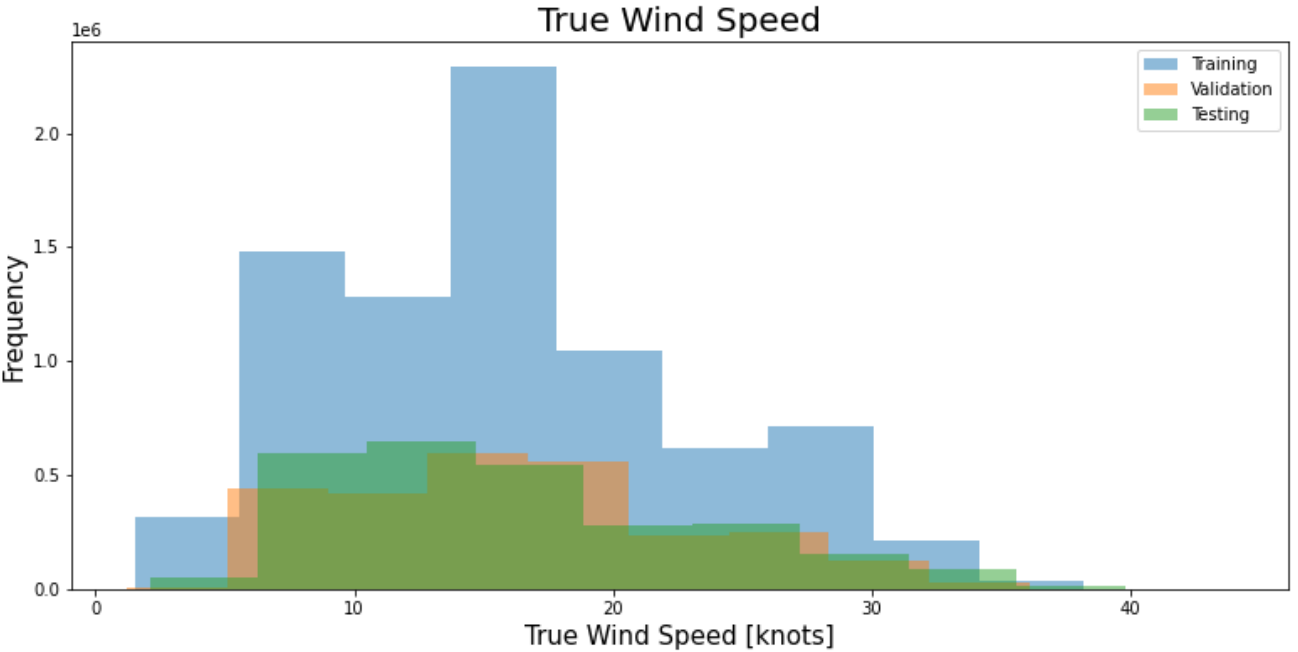
\includegraphics[width = \hsize]{figures/distributions/atlantic-TWS.png}
\caption{Distribution of True Wind Speed in \textit{Atlantic} dataset \cite{charles}}
\label{fig:atlantic-tws}
\end{figure}

\begin{figure}[h]
     \centering
     \begin{subfigure}[t]{0.49\textwidth}
         \centering
         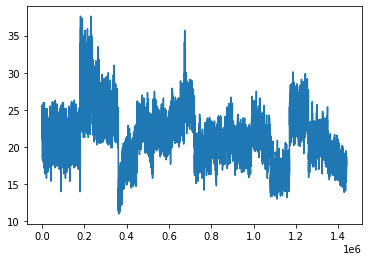
\includegraphics[width=\textwidth]{figures/distributions/RDR-TWS.png}
         \caption{RDR\_nkz}
     \end{subfigure}
     \hfill
     \begin{subfigure}[t]{0.49\textwidth}
         \centering
         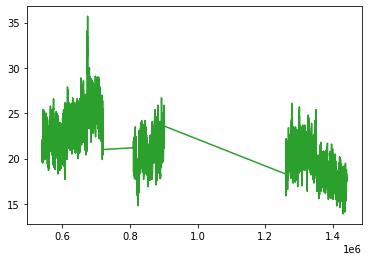
\includegraphics[width=\textwidth]{figures/distributions/RDR-atlantic-TWS.png}
         \caption{RDR\_nkz (Atlantic Conditions)}
     \end{subfigure}
        \label{fig:rdr-tws}
        \caption{True Wind Speed plots}
\end{figure}

\clearpage
\subsubsection{True Wind Angle (TWA)}
Again, pretty much all wind angles are covered in training data. However, we have less data from +150 compared to 50 and -150.
To exclude +150 range, Remaining good candidates are:
\begin{itemize}
    \item start-0.45
    \item 0.55-0.75*
    \item 0.8-0.9*
    \item 1.25-end*
\end{itemize}
The candidates that are suitable for all features are shown with a star(*).

\begin{figure}[h]
\centering
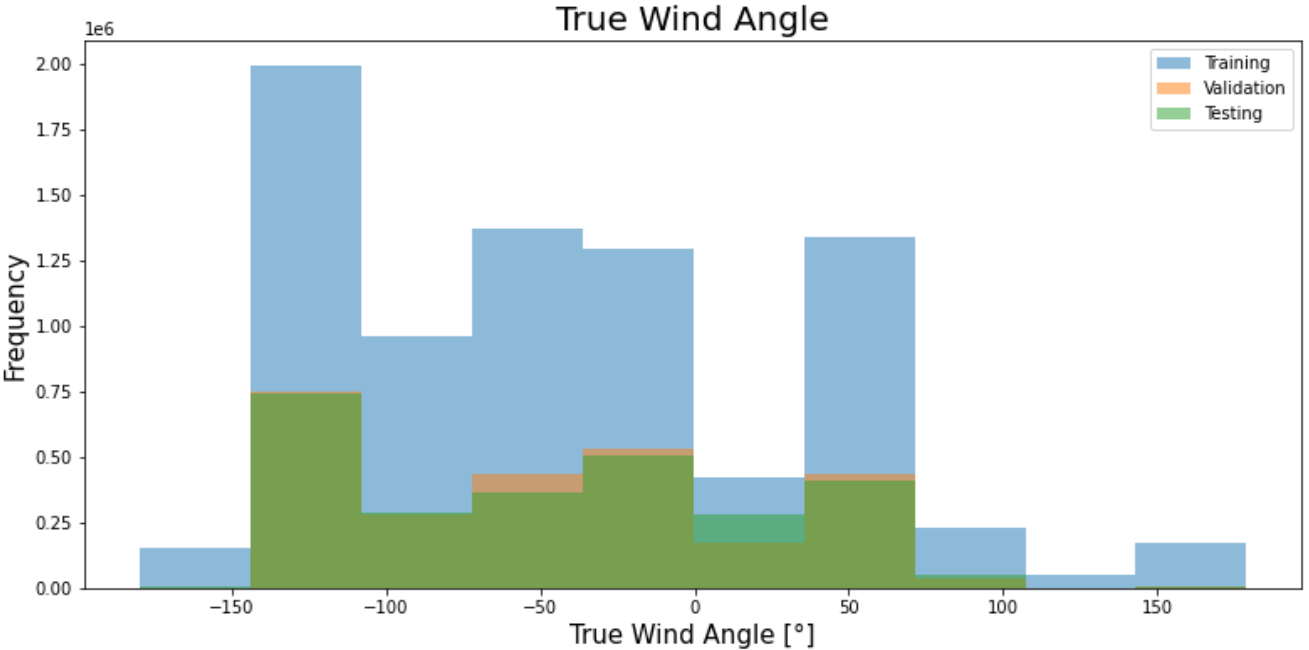
\includegraphics[width = \hsize]{figures/distributions/atlantic-TWA.png}
\caption{Distribution of True Wind Angle in \textit{Atlantic} dataset \cite{charles}}
\label{fig:atlantic-tws}
\end{figure}

\begin{figure}[h]
     \centering
     \begin{subfigure}[t]{0.49\textwidth}
         \centering
         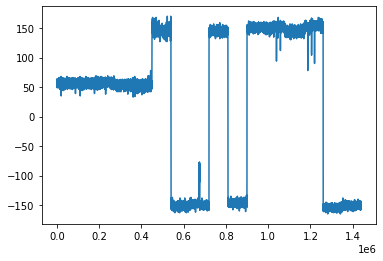
\includegraphics[width=\textwidth]{figures/distributions/RDR-TWA.png}
         \caption{RDR\_nkz}
     \end{subfigure}
     \hfill
     \begin{subfigure}[t]{0.49\textwidth}
         \centering
         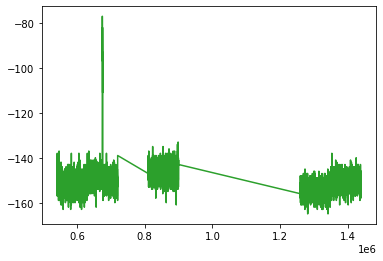
\includegraphics[width=\textwidth]{figures/distributions/RDR-atlantic-TWA.png}
         \caption{RDR\_nkz (Atlantic Conditions)}
     \end{subfigure}
        \label{fig:rdr-tws}
        \caption{True Wind Angle plots}
\end{figure}

\clearpage
\subsubsection{Apparent Wind Angle (AWA)}
All of the apparent wind angles in \textit{RDR\_nkz} are covered in training data.

\begin{figure}[h]
\centering
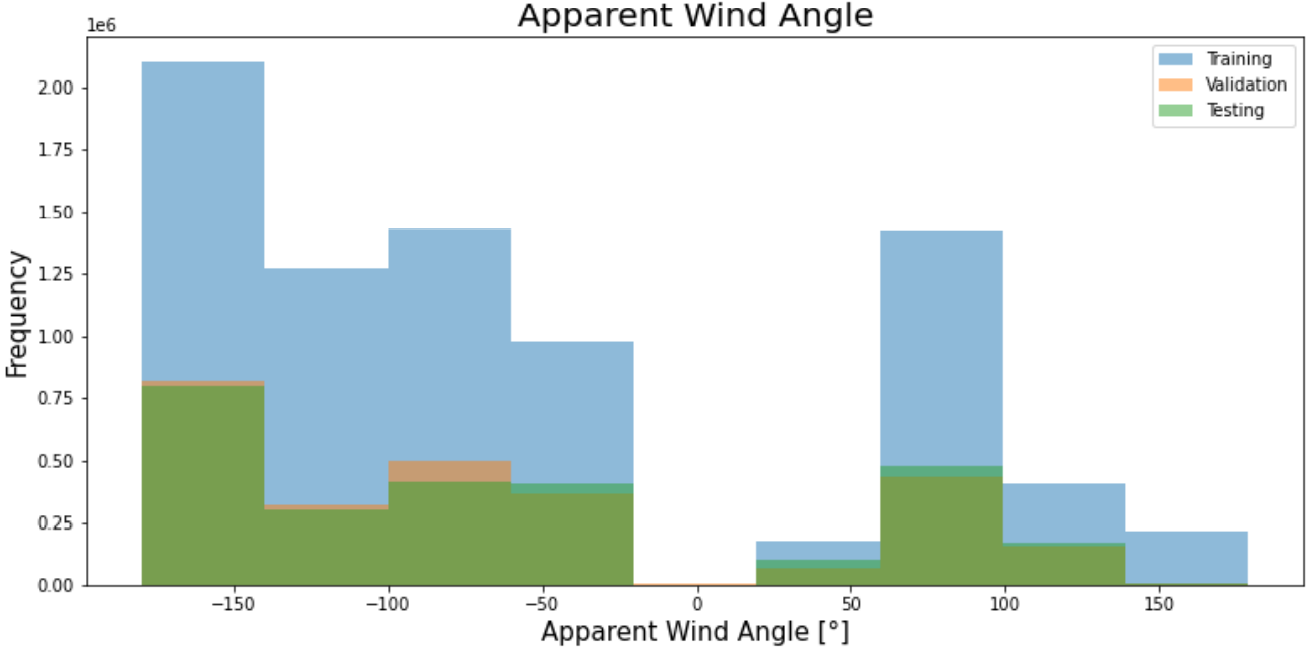
\includegraphics[width = \hsize]{figures/distributions/atlantic-AWA.png}
\caption{Distribution of Apparent Wind Angle in \textit{Atlantic} dataset \cite{charles}}
\label{fig:atlantic-tws}
\end{figure}

\begin{figure}[h]
     \centering
     \begin{subfigure}[t]{0.49\textwidth}
         \centering
         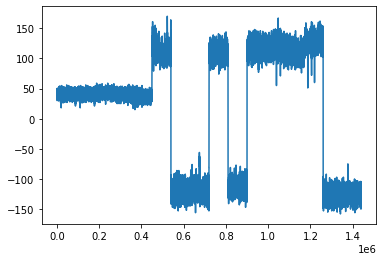
\includegraphics[width=\textwidth]{figures/distributions/RDR-AWA.png}
         \caption{RDR\_nkz}
     \end{subfigure}
     \hfill
     \begin{subfigure}[t]{0.49\textwidth}
         \centering
         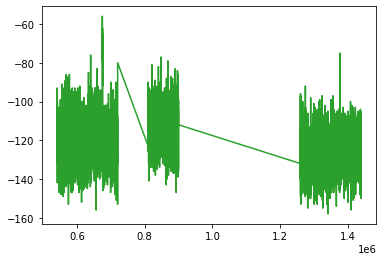
\includegraphics[width=\textwidth]{figures/distributions/RDR-atlantic-AWA.png}
         \caption{RDR\_nkz (Atlantic Conditions)}
     \end{subfigure}
        \label{fig:rdr-tws}
        \caption{Apparent Wind Angle plots}
\end{figure}

\clearpage
\subsubsection{Pitch}
We want Pitch to be mostly between 0 and 15. Good candidates for this range:
\begin{itemize}
    \item 0.55-0.7*
    \item 0.8-0.9*
    \item 1.25-end*
\end{itemize}
The candidates that are suitable for all features are shown with a star(*).

\begin{figure}[h]
\centering
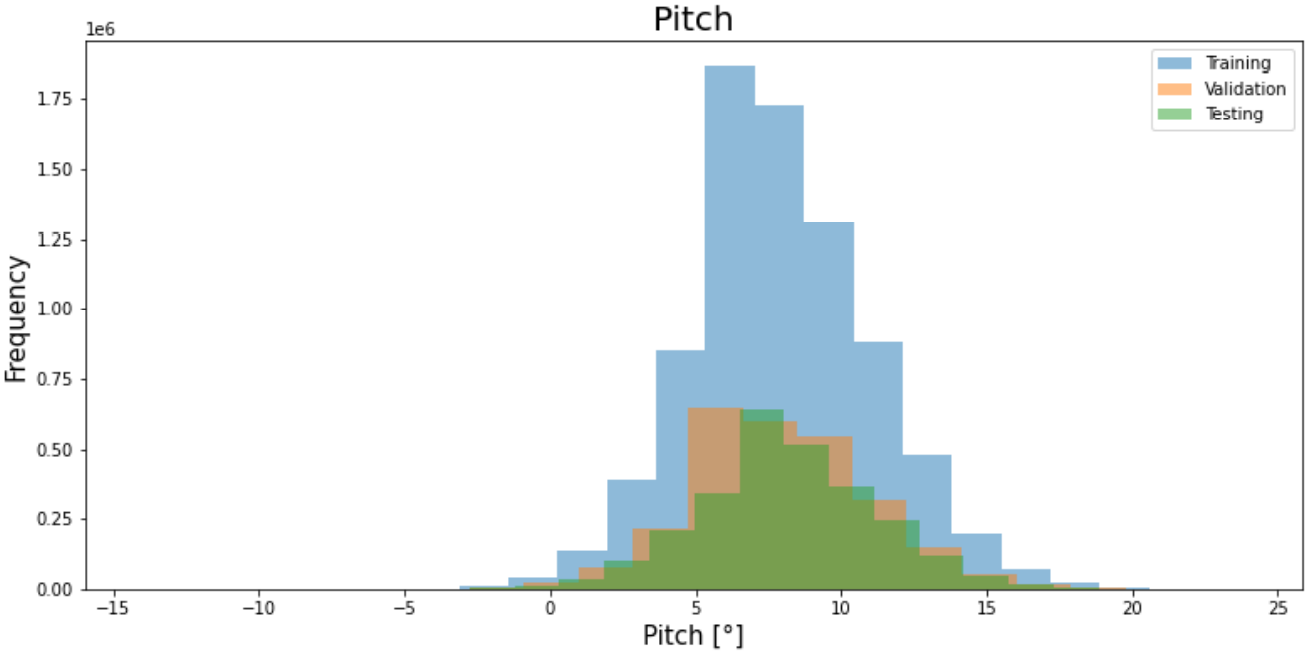
\includegraphics[width = \hsize]{figures/distributions/atlantic-Pitch.png}
\caption{Distribution of Pitch in \textit{Atlantic} dataset \cite{charles}}
\label{fig:atlantic-tws}
\end{figure}

\begin{figure}[h]
     \centering
     \begin{subfigure}[t]{0.49\textwidth}
         \centering
         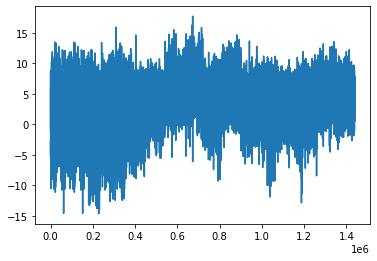
\includegraphics[width=\textwidth]{figures/distributions/RDR-Pitch.png}
         \caption{RDR\_nkz}
     \end{subfigure}
     \hfill
     \begin{subfigure}[t]{0.49\textwidth}
         \centering
         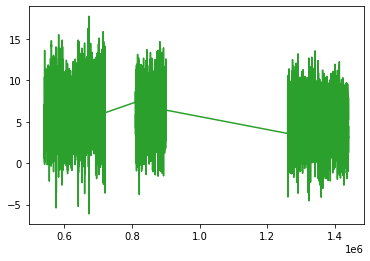
\includegraphics[width=\textwidth]{figures/distributions/RDR-atlantic-Pitch.png}
         \caption{RDR\_nkz (Atlantic Conditions)}
     \end{subfigure}
        \label{fig:rdr-tws}
        \caption{Pitch plots}
\end{figure}
